% SECTION ====================================================================================
\section{AVL Bäume}
% ============================================================================================

\begin{sectionbox}
\textbf{Ziel}: Verhinderung der Degenerierung $\rightarrow$ garantiere, dass ein Baum mit $n$ Knoten stets eine Höhe von $\mathcal{O}(\operatorname{log}(n))$.\par\smallskip
\subsection{AVL Bedingung}\smallskip
\subsubsection{Balance eines Knotens}\smallskip
Die Balance eines Knotens $v$ ist definiert als die Höhendifferenz seiner beiden Teilbäume $T_{l}(v)$ und $T_{r}(v)$:\par\smallskip
\begin{center}
    $\operatorname{bal}(v):=h\left(T_{r}(v)\right)-h\left(T_{l}(v)\right)$
\end{center}\par\smallskip
\begin{itemize}
    \item \textbf{Augmentieren}: $v.size$ Feld mit \textbf{Balance}
    \item \textbf{Baumhöhe}: Ein AVL Baum ist asymptotisch nicht mehr als 44\% höher als ein perfekt balancierter Baum ($\left\lceil\log _{2} n+1\right\rceil$).
\end{itemize}\par\smallskip

\subsubsection{AVL Bedingung}\smallskip
AVL Bedingung: für \textit{jeden} Knoten $v$ eines Baumes gilt:\par\smallskip
\begin{center}
    $\operatorname{bal}(v) \in\{-1,0,1\}$
\end{center}\par\smallskip

\textit{Beispiele}\par
\begin{center}
    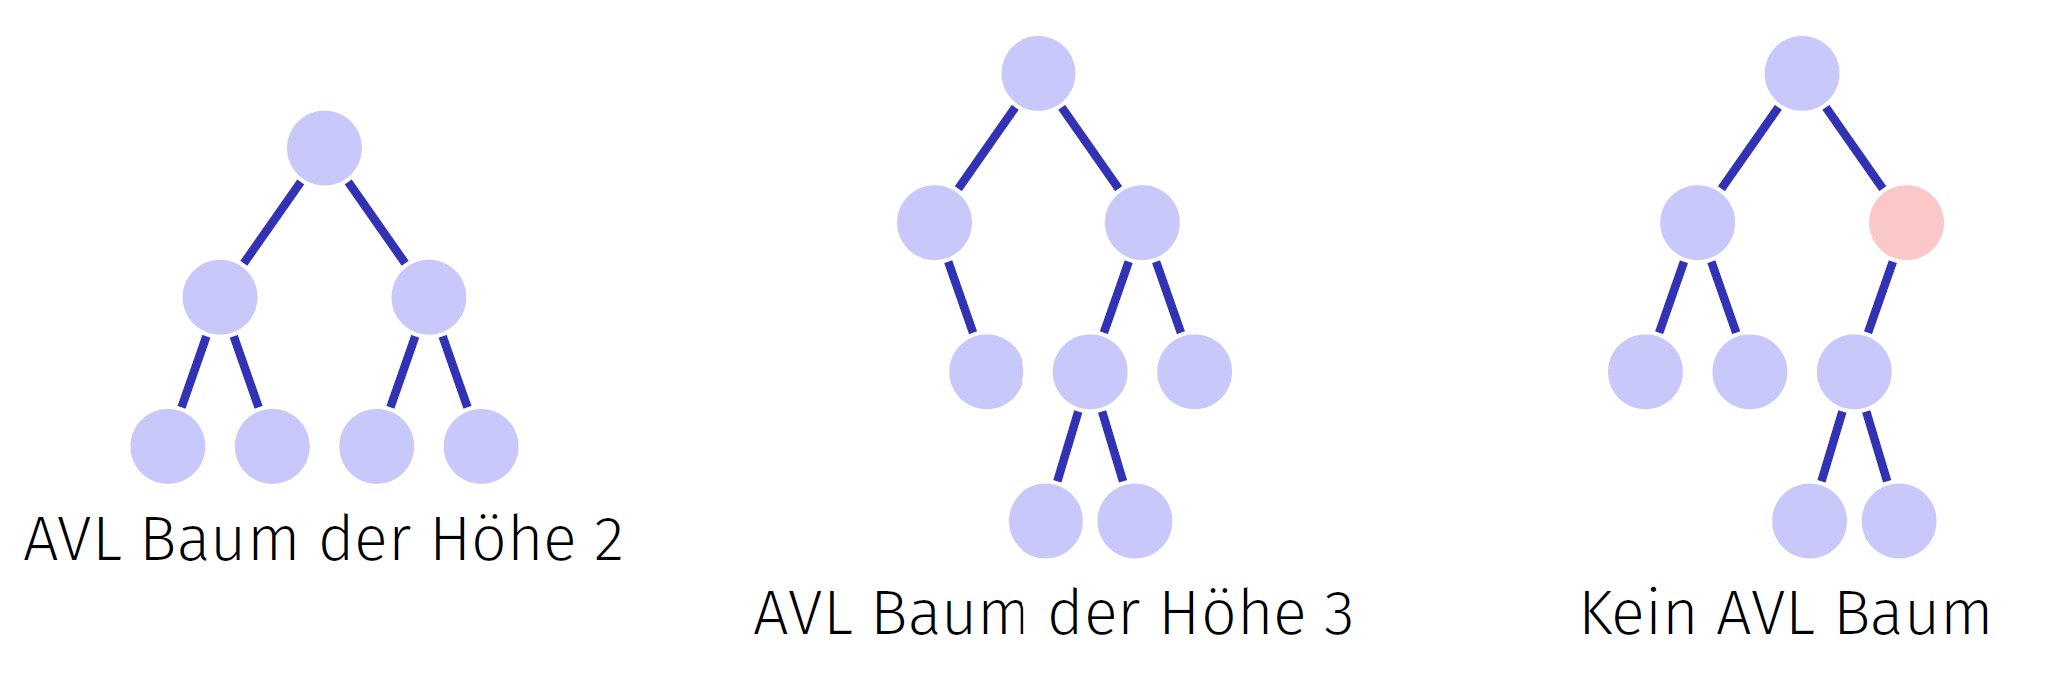
\includegraphics[width = \columnwidth]{../img/BspAVLHoehen.png}
\end{center}

\end{sectionbox}

\begin{sectionbox}
\subsection{Einfügen}\smallskip
\begin{itemize}
    \item Zuerst einfügen wie bei Suchbaum.
    \item Prüfe die Balance-Bedingung für alle Knoten aufsteigend von n zur Wurzel.
    \par \textbf{$\operatorname{upin}(p)$}: Aufsteigend von $p$ die Balance (Augmentation) anpassen, wobei gilt $\operatorname{bal}(p) \in \{-1,0,+1\}$.
    \item Problematischer Fall (rebalancieren!): $p$ ist linker Sohn von $pp$, wobei $\operatorname{bal}(pp)$ bereits vor dem Einfügen $-1$ ist (danach $-2$).
\end{itemize}\par\smallskip
\end{sectionbox}

\begin{sectionbox}
\subsection{Rebalancieren: Rotationen}\smallskip
\textit{Fall 1: Rotation nach rechts}\par
\begin{center}
    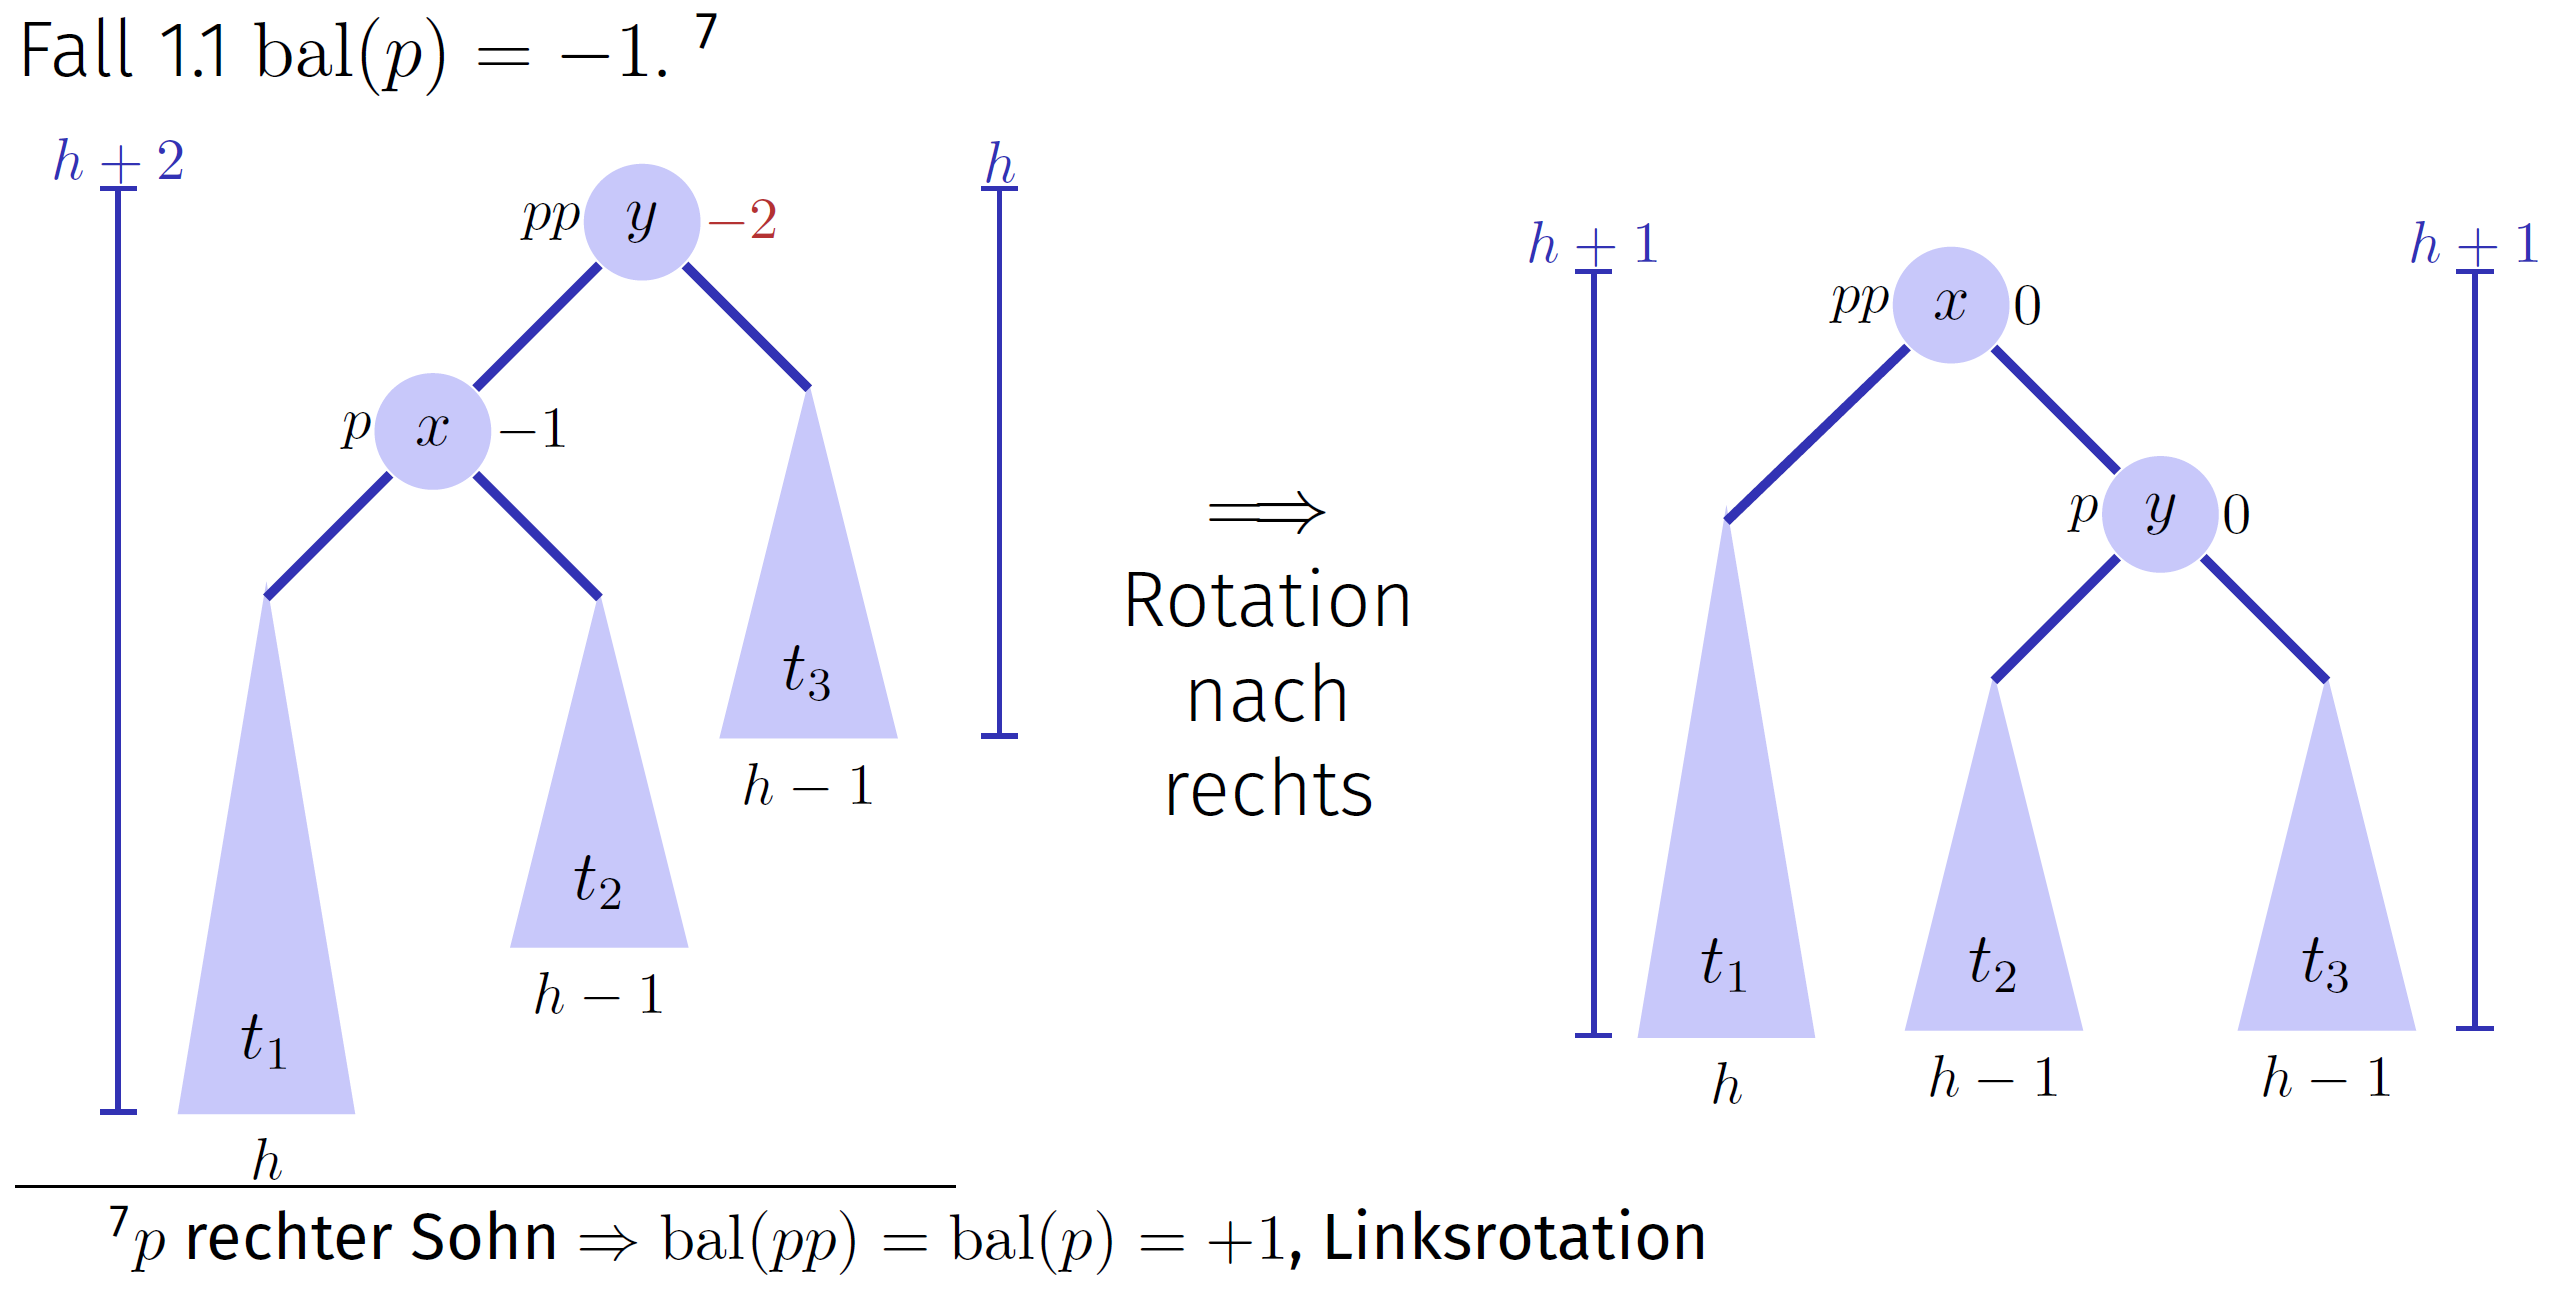
\includegraphics[width = \columnwidth]{../img/rotR.png}
\end{center}\smallskip
\textit{Fall 2: Doppelrotation nach links-rechts}\par
\begin{center}
    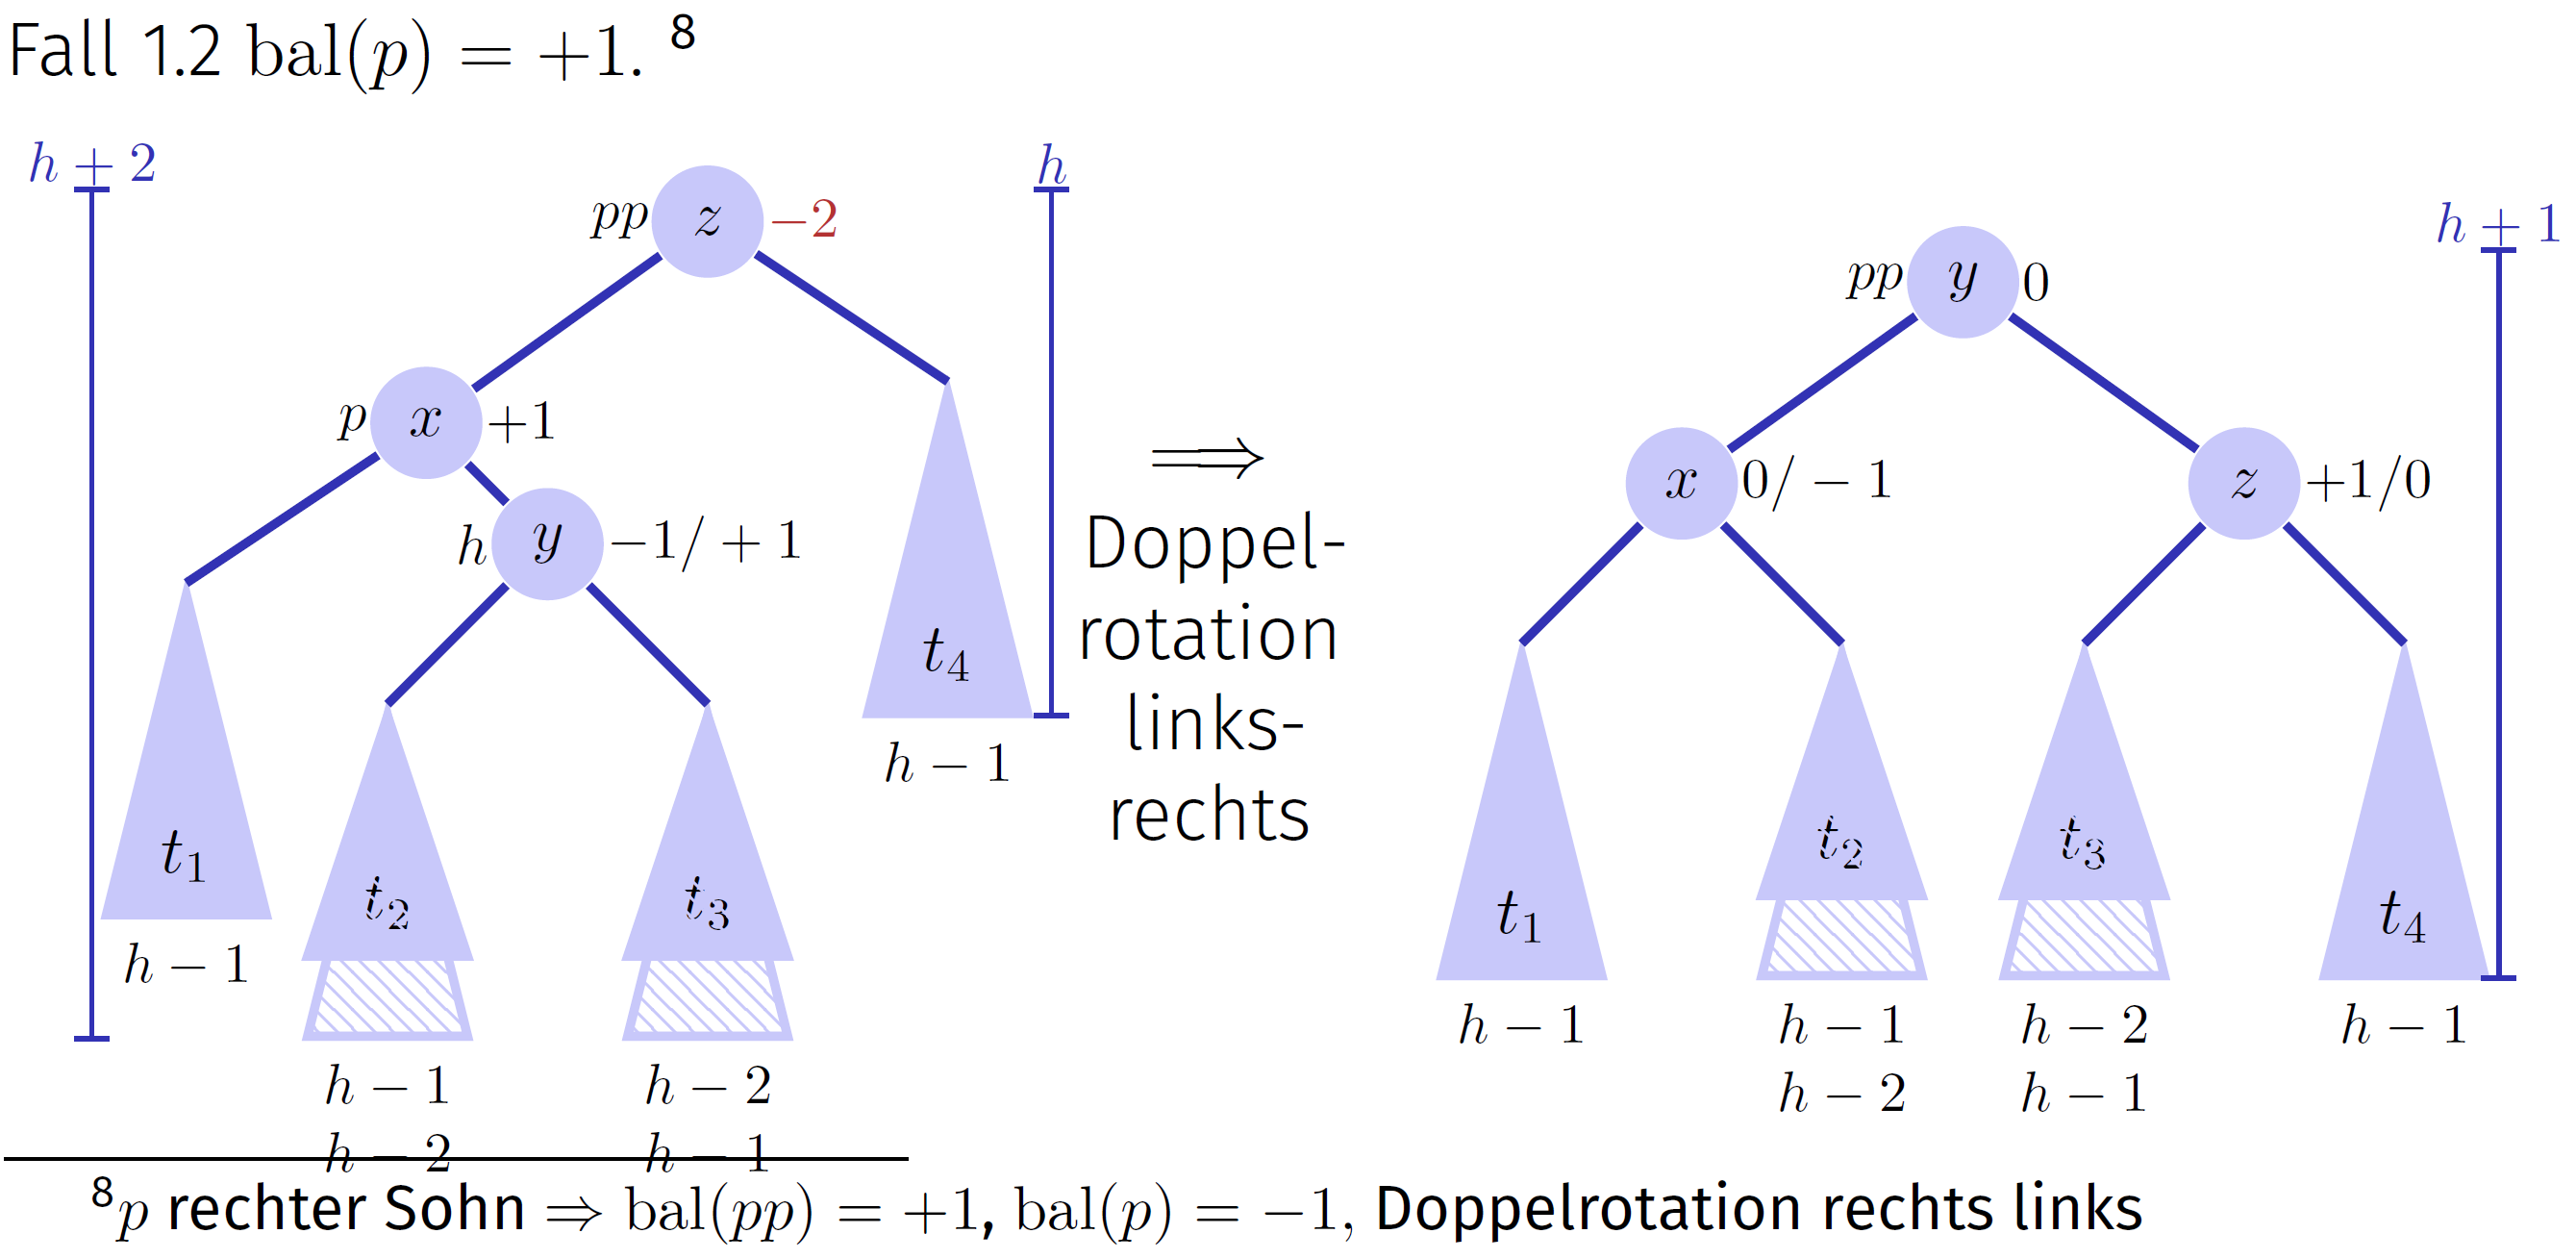
\includegraphics[width = \columnwidth]{../img/rotLR.png} \par\smallskip
    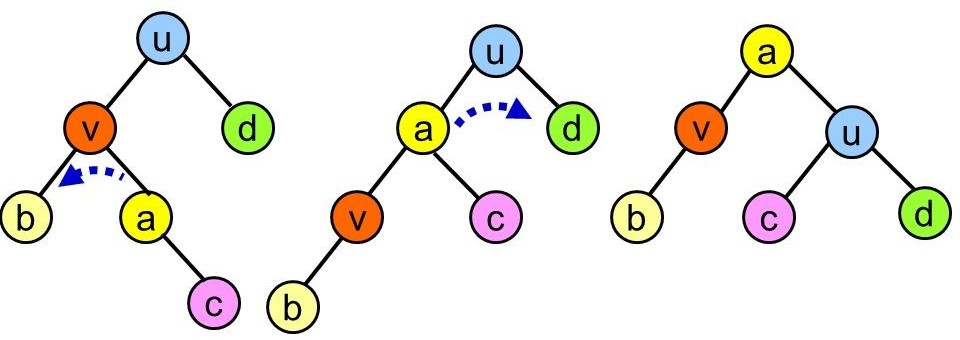
\includegraphics[width = \columnwidth]{../img/Doppelrotationen.jpg}
\end{center}\smallskip
\end{sectionbox}

\begin{sectionbox}
\subsection{Analyse}\smallskip
AVL-Bäume haben asymptotische Laufzeit von $\mathcal{O}(\operatorname{log}(n))$ (schlechtester Fall) für das Suchen, Einfügen und Löschen von Schlüsseln. Einfügen und Löschen ist verhältnismässig aufwändig und für kleine Probleme relativ langsam.
\end{sectionbox}


% TODO: what is this?
\begin{sectionbox}
\subsection{Beispiel: Augmentierter SearchNode}\smallskip
\begin{lstlisting}[language=Python]
class SearchNode(object):
  def __init__(self, k):
    self.key = k
    self.left = self.right = None
    self.size = 1       # Augmentiere Hoehe mit 1
\end{lstlisting}\vspace{-6px}
\end{sectionbox}